\documentclass{article}

\usepackage[preprint]{neurips_2025}

\usepackage[utf8]{inputenc}
\usepackage[T1]{fontenc}
\usepackage{hyperref}
\usepackage{url}
\usepackage{booktabs}
\usepackage{graphicx}
\usepackage{amsmath}
\usepackage{microtype}
\usepackage{xcolor}

\title{DistilBERT vs. BERT for Efficient Text Classification}

\author{%
  Arturo Rivas\\
  NLP Text Classification Project\\
  \texttt{TODO: add institutional email if needed}
}

\begin{document}

\maketitle

\begin{abstract}
This mini-report studies the accuracy-efficiency trade-off between DistilBERT and BERT-base for text classification on AG News, SST-2, and Yelp Review Full. We fine-tune DistilBERT, run a DistilBERT-only ablation over classifier heads and freezing strategies, select the best DistilBERT configuration per dataset, and compare it with BERT-base. Evaluation uses accuracy, macro and weighted precision, recall, and F1, plus efficiency metrics including parameter count, latency, and peak GPU memory when available. The report is generated from saved experiment artifacts; debug-fast numbers are placeholders for pipeline validation and must be replaced by full-run results before drawing final conclusions.
\end{abstract}

\section{Introduction}
Text classification is a core natural language processing task with applications in topic classification, sentiment analysis, and review understanding. Transformer encoders such as BERT provide strong transfer learning performance by pretraining deep bidirectional representations \citep{devlin2019bert}. However, BERT-base is comparatively expensive in parameter count, memory, and inference latency, which can be limiting for deployment.

DistilBERT is a compressed Transformer model trained by knowledge distillation to retain much of BERT's language understanding ability with fewer parameters and faster inference \citep{sanh2019distilbert}. This project asks whether DistilBERT can offer a favorable trade-off against BERT-base on three classification datasets: AG News, SST-2 from GLUE, and Yelp Review Full \citep{zhang2015character,wang2018glue}.

The contributions are: (1) a reproducible data and training pipeline for DistilBERT and BERT-base; (2) a DistilBERT ablation over classifier size and freezing strategies; (3) a final comparison of the selected DistilBERT configuration against BERT-base; and (4) a compact analysis of performance and efficiency metrics.

\section{Approach}
All datasets are tokenized with the corresponding Hugging Face tokenizer and padded/truncated to a maximum sequence length of 128. The primary training objective is cross-entropy loss over dataset labels. For DistilBERT, the baseline keeps the Transformer encoder fully trainable and uses the standard classification head. The ablation study additionally evaluates a fully frozen Transformer, smaller and larger multilayer classifier heads, and a partial-freezing strategy that freezes embeddings and lower Transformer layers.

BERT-base uses \texttt{bert-base-uncased} with a comparable sequence classification head where possible. The model builder handles architecture-specific module names for DistilBERT and BERT, including embeddings and Transformer layer freezing. Models are evaluated using accuracy, macro precision/recall/F1, and weighted precision/recall/F1. Efficiency is measured using total parameters, trainable parameters, latency in milliseconds per sample, and peak GPU memory when CUDA measurements are available.

\section{Experiments}
The datasets cover topic classification (AG News), binary sentiment classification (SST-2), and five-class review rating prediction (Yelp Review Full). The default fine-tuning setup uses AdamW through the Hugging Face Trainer, learning rate $2\times10^{-5}$, weight decay 0.01, maximum length 128, and three epochs for full runs. Debug-fast mode uses tiny subsets and very few optimizer steps only to validate code paths.

The implementation uses PyTorch, Hugging Face Transformers, and Hugging Face Datasets \citep{paszke2019pytorch,wolf2020transformers,lhoest2021datasets}. Full-run experiments are intended for the target RTX 4090 environment with mixed precision enabled when CUDA is available. Debug-fast artifacts may appear in the generated tables if full-run results have not been produced; those values should not be interpreted as final experimental evidence.

\section{Analysis}
Table~\ref{tab:performance} summarizes final performance for the selected DistilBERT configuration and BERT-base. Table~\ref{tab:efficiency} reports efficiency metrics. Table~\ref{tab:ablation} gives a compact ablation summary, and Table~\ref{tab:best-distilbert} lists the selected DistilBERT configuration per dataset.

\begin{table}[t]
\centering
\caption{Final performance comparison. Metrics are generated from \texttt{results/tables/final\_performance\_table.csv}.}
\label{tab:performance}
\resizebox{\linewidth}{!}{\begin{tabular}{lllrrrrrrr}
\toprule
Dataset & Model & Config & Acc. & Prec. & Rec. & F1 & Prec. w. & Rec. w. & F1 w. \\
\midrule
ag\_news & distilbert & large\_classifier & 0.9393 & 0.9395 & 0.9393 & 0.9394 & 0.9395 & 0.9393 & 0.9394 \\
ag\_news & bert & bert\_base & 0.9462 & 0.9463 & 0.9462 & 0.9461 & 0.9463 & 0.9462 & 0.9461 \\
sst2 & distilbert & large\_classifier & 0.9106 & 0.9105 & 0.9106 & 0.9105 & 0.9106 & 0.9106 & 0.9106 \\
sst2 & bert & bert\_base & 0.9209 & 0.9208 & 0.9209 & 0.9208 & 0.9209 & 0.9209 & 0.9209 \\
yelp\_review\_full & distilbert & baseline & 0.6503 & 0.6508 & 0.6503 & 0.6502 & 0.6508 & 0.6503 & 0.6502 \\
yelp\_review\_full & bert & bert\_base & 0.6576 & 0.6577 & 0.6576 & 0.6575 & 0.6577 & 0.6576 & 0.6575 \\
\bottomrule
\end{tabular}
}
\end{table}

\begin{table}[t]
\centering
\caption{Final efficiency comparison. Parameter counts are shown in millions. Latency is in ms/sample.}
\label{tab:efficiency}
\resizebox{\linewidth}{!}{\begin{tabular}{lllrrrr}
\toprule
Dataset & Model & Config & Params (M) & Trainable (M) & Latency & GPU MB \\
\midrule
ag\_news & distilbert & freeze\_lower\_layers & 66.56 & 21.46 & 109.25 & -- \\
ag\_news & bert & bert\_base & 109.49 & 109.49 & 245.26 & -- \\
sst2 & distilbert & freeze\_lower\_layers & 66.56 & 21.46 & 101.88 & -- \\
sst2 & bert & bert\_base & 109.48 & 109.48 & 313.31 & -- \\
yelp\_review\_full & distilbert & small\_classifier & 66.46 & 66.46 & 116.33 & -- \\
yelp\_review\_full & bert & bert\_base & 109.49 & 109.49 & 320.41 & -- \\
\bottomrule
\end{tabular}
}
\end{table}

\begin{figure}[t]
\centering
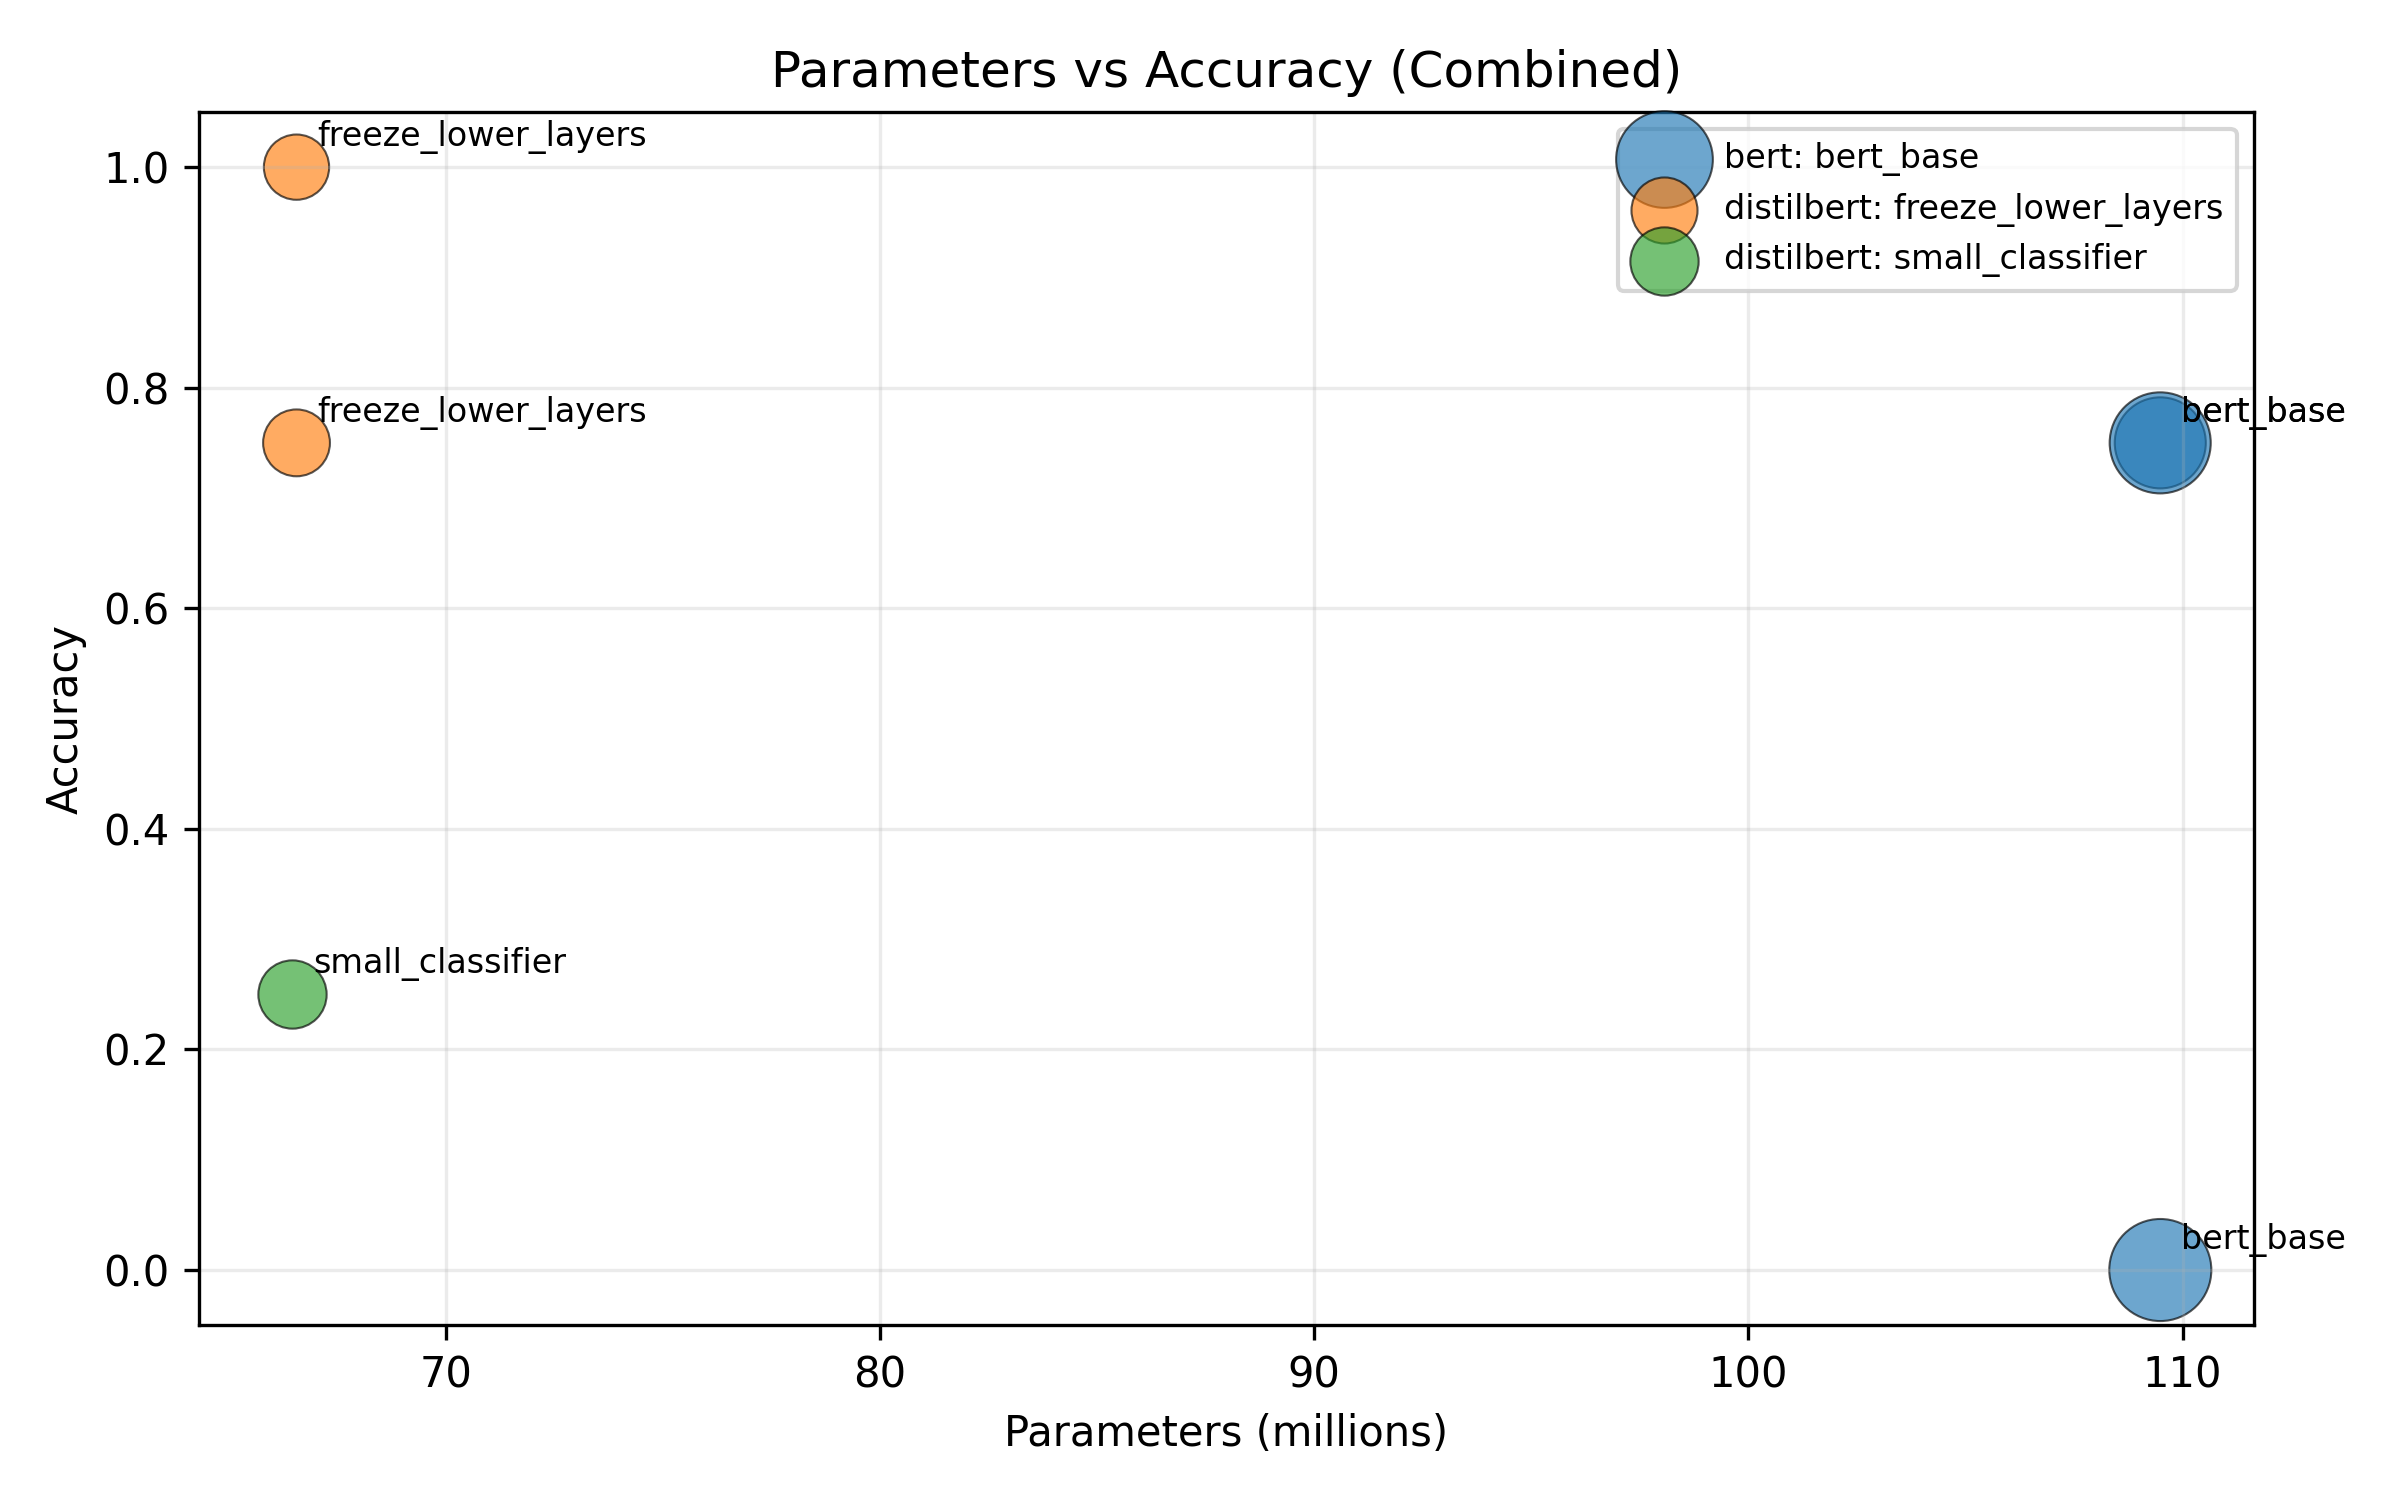
\includegraphics[width=0.78\linewidth]{figures/bubble_params_accuracy_combined.png}
\caption{Accuracy versus parameter count. Bubble size uses latency when available, otherwise memory.}
\label{fig:bubble}
\end{figure}

\begin{figure}[t]
\centering
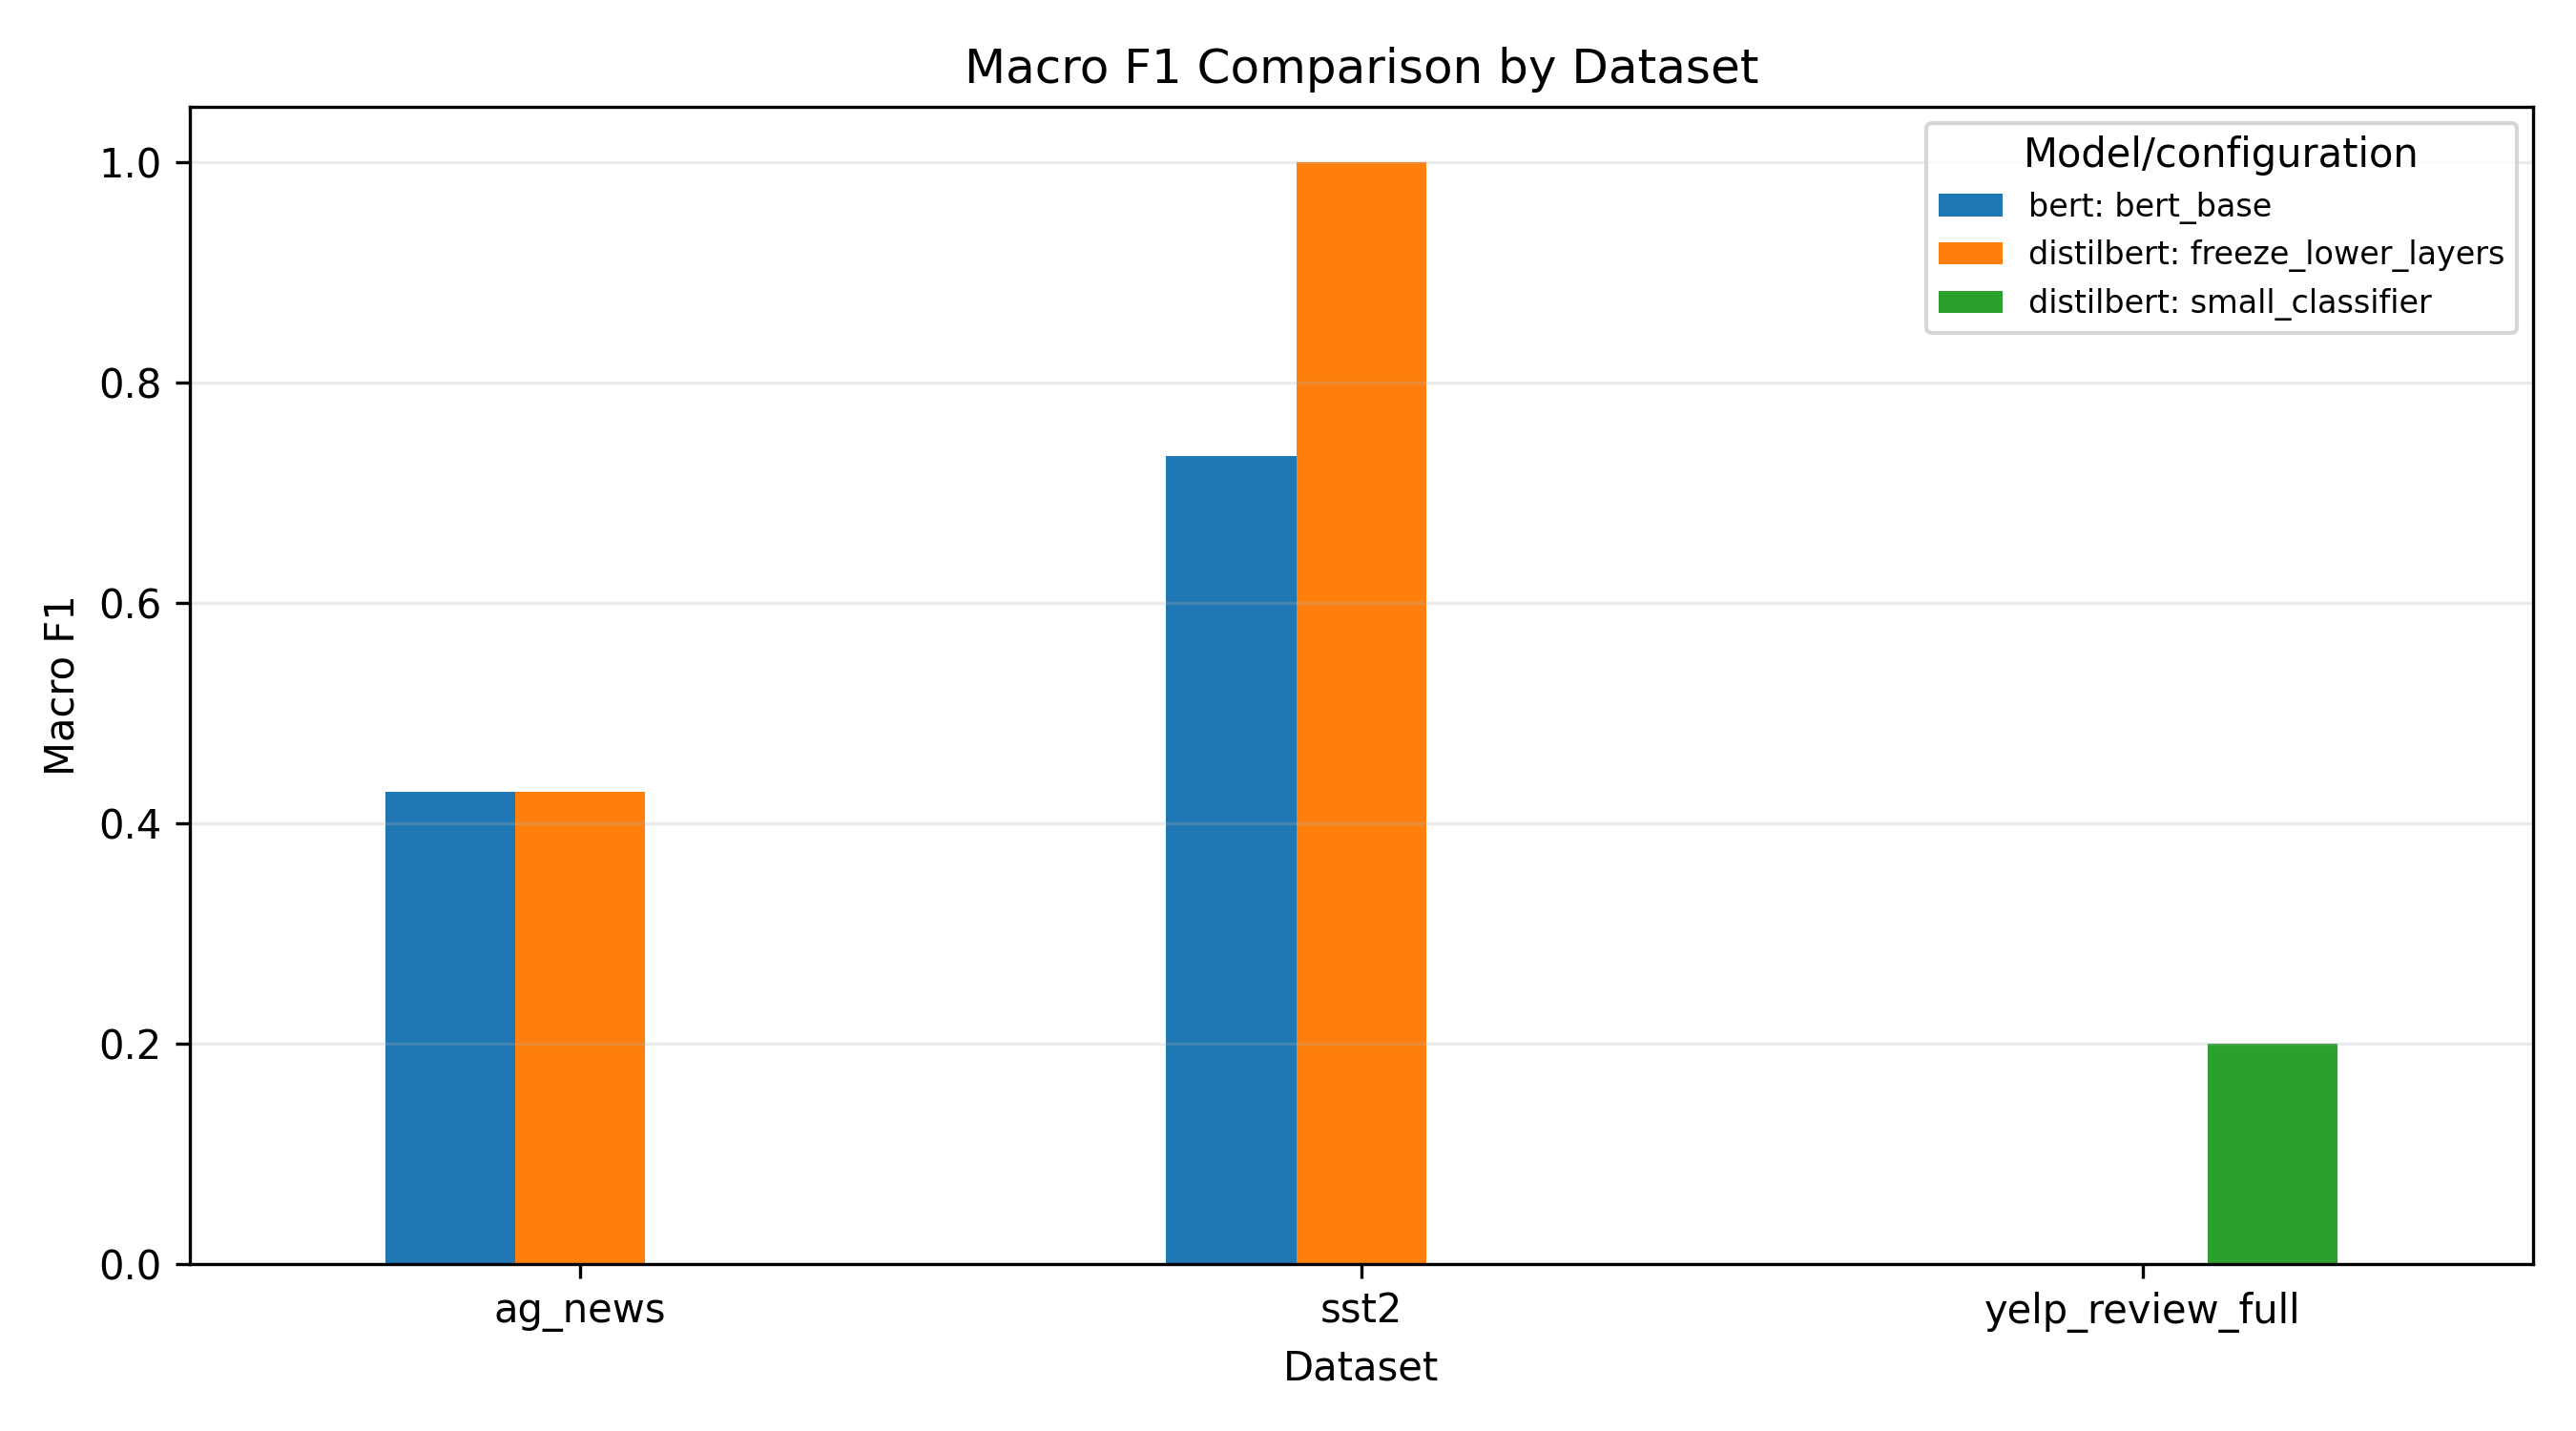
\includegraphics[width=0.48\linewidth]{figures/f1_comparison_by_dataset.png}
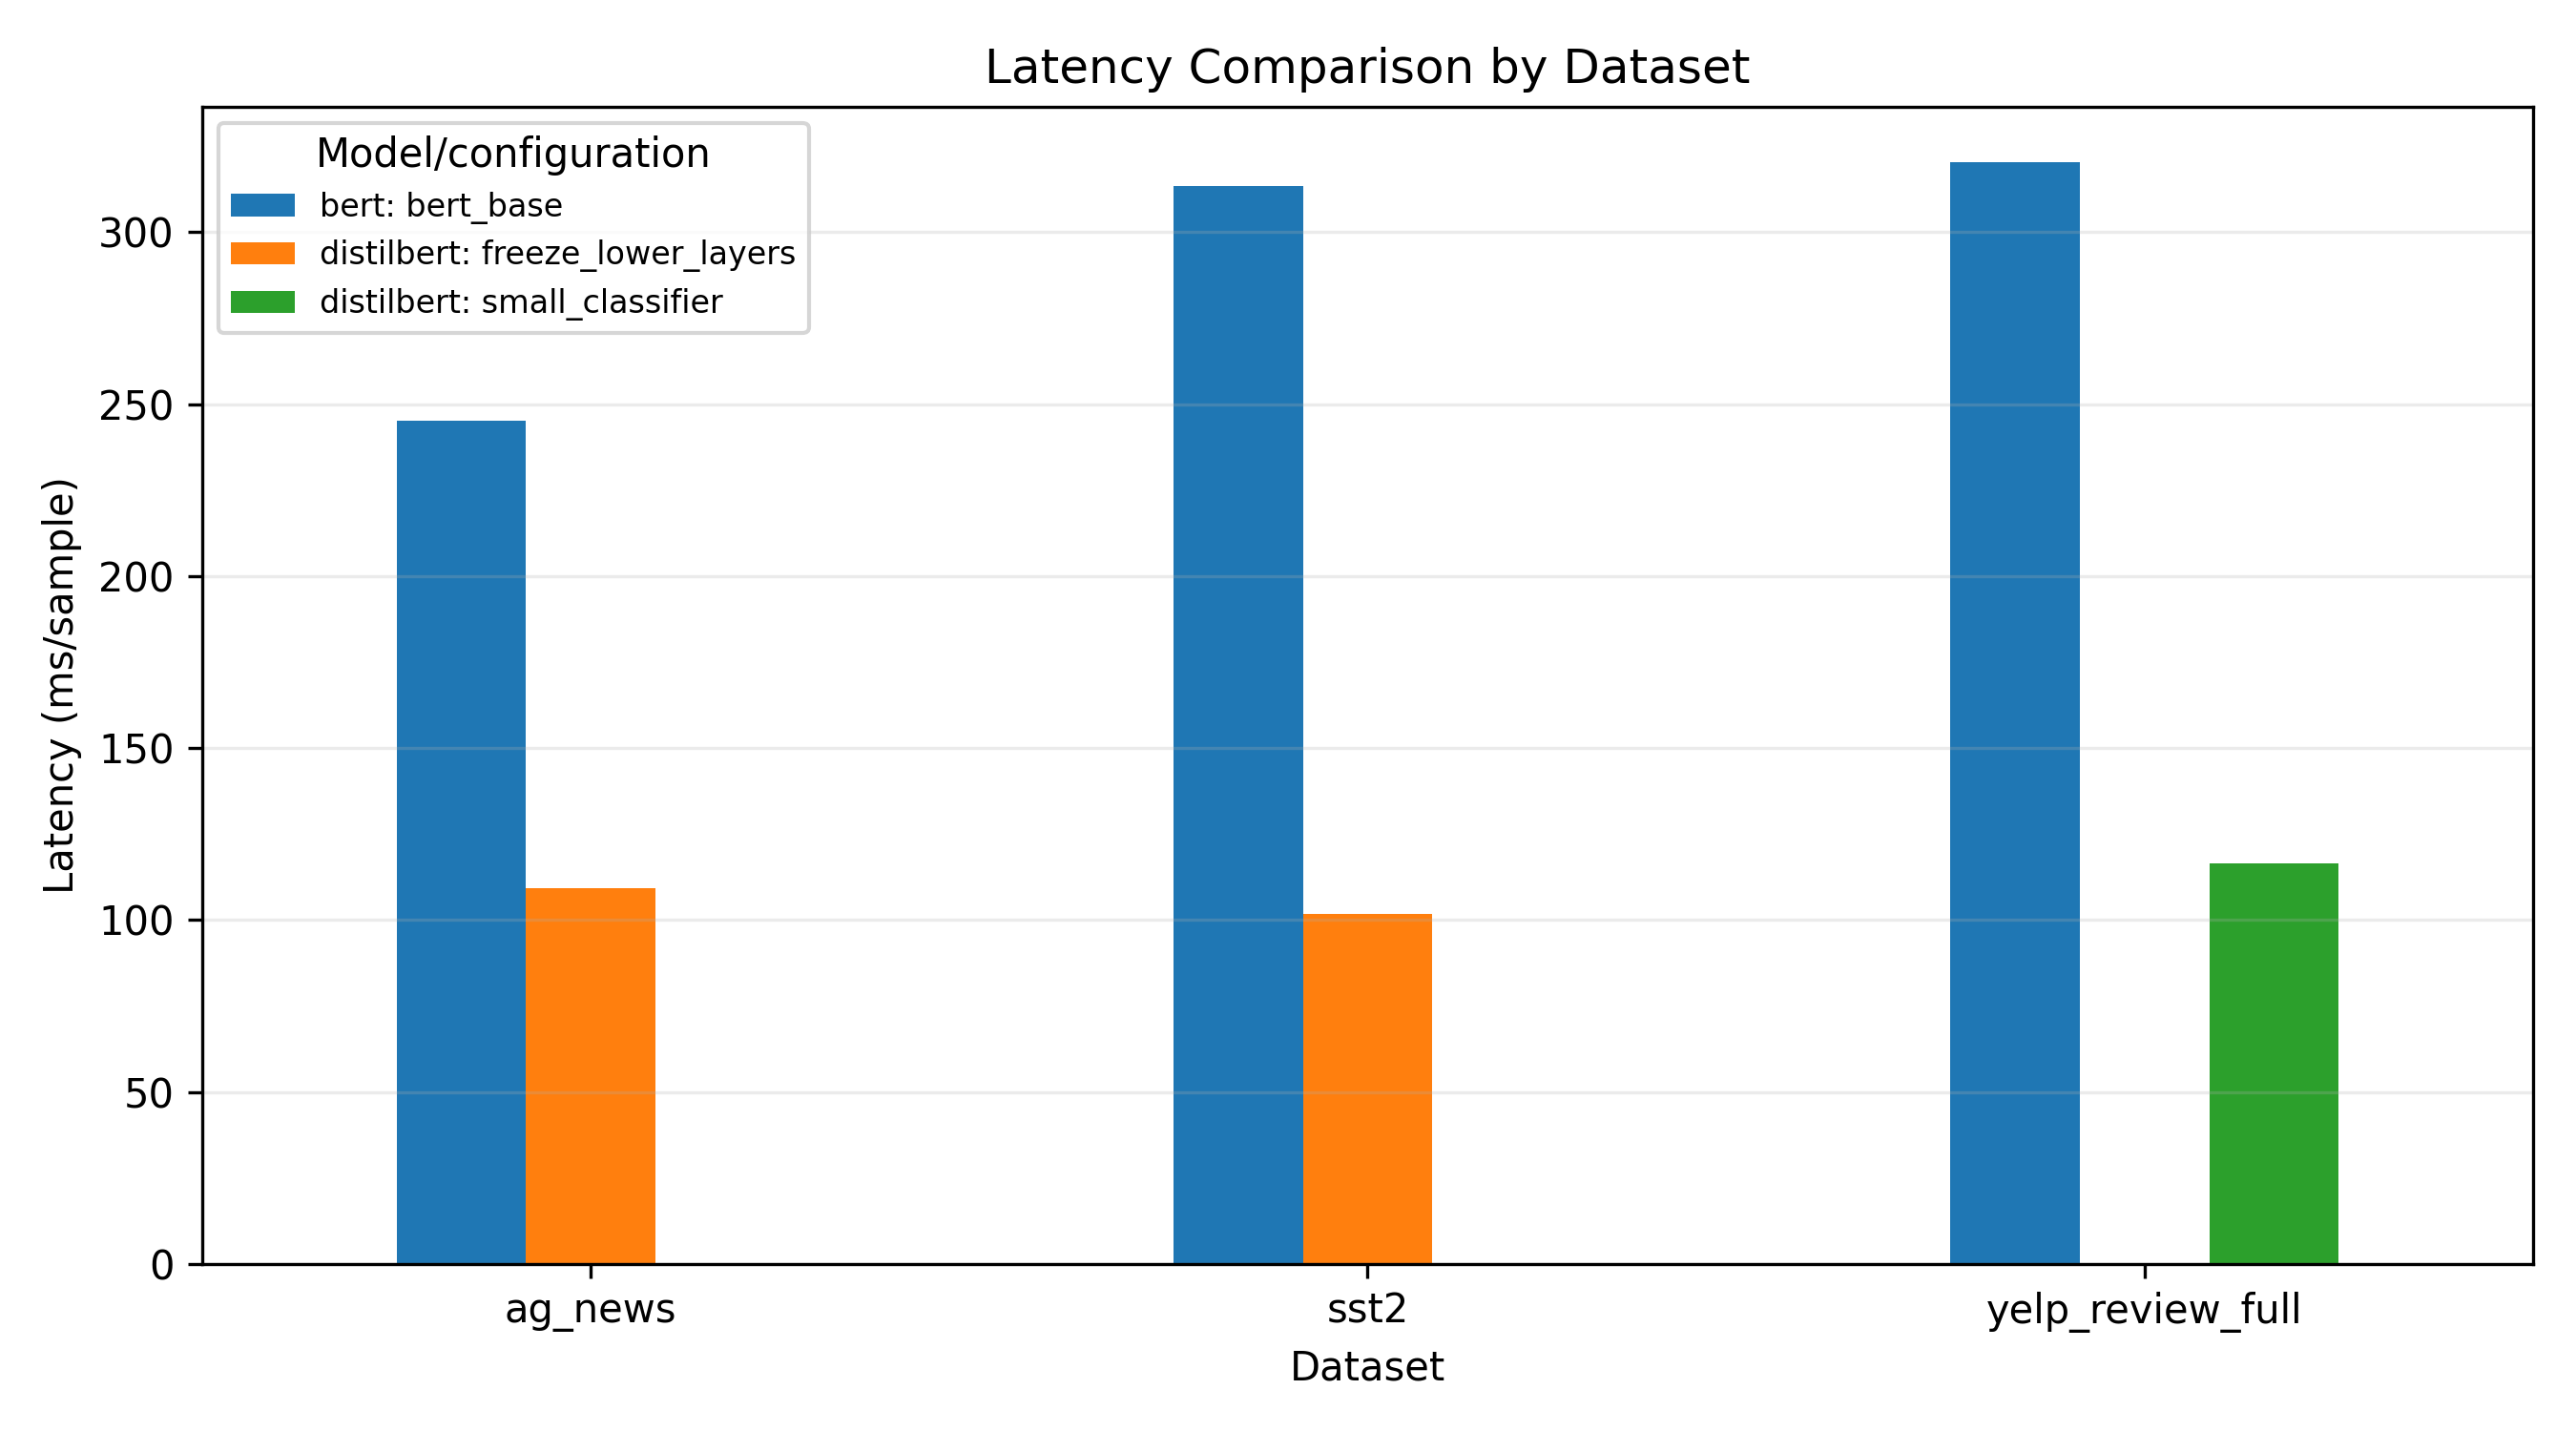
\includegraphics[width=0.48\linewidth]{figures/latency_comparison_by_dataset.png}
\caption{Macro F1 and latency comparison by dataset.}
\label{fig:f1-latency}
\end{figure}

\begin{figure}[t]
\centering
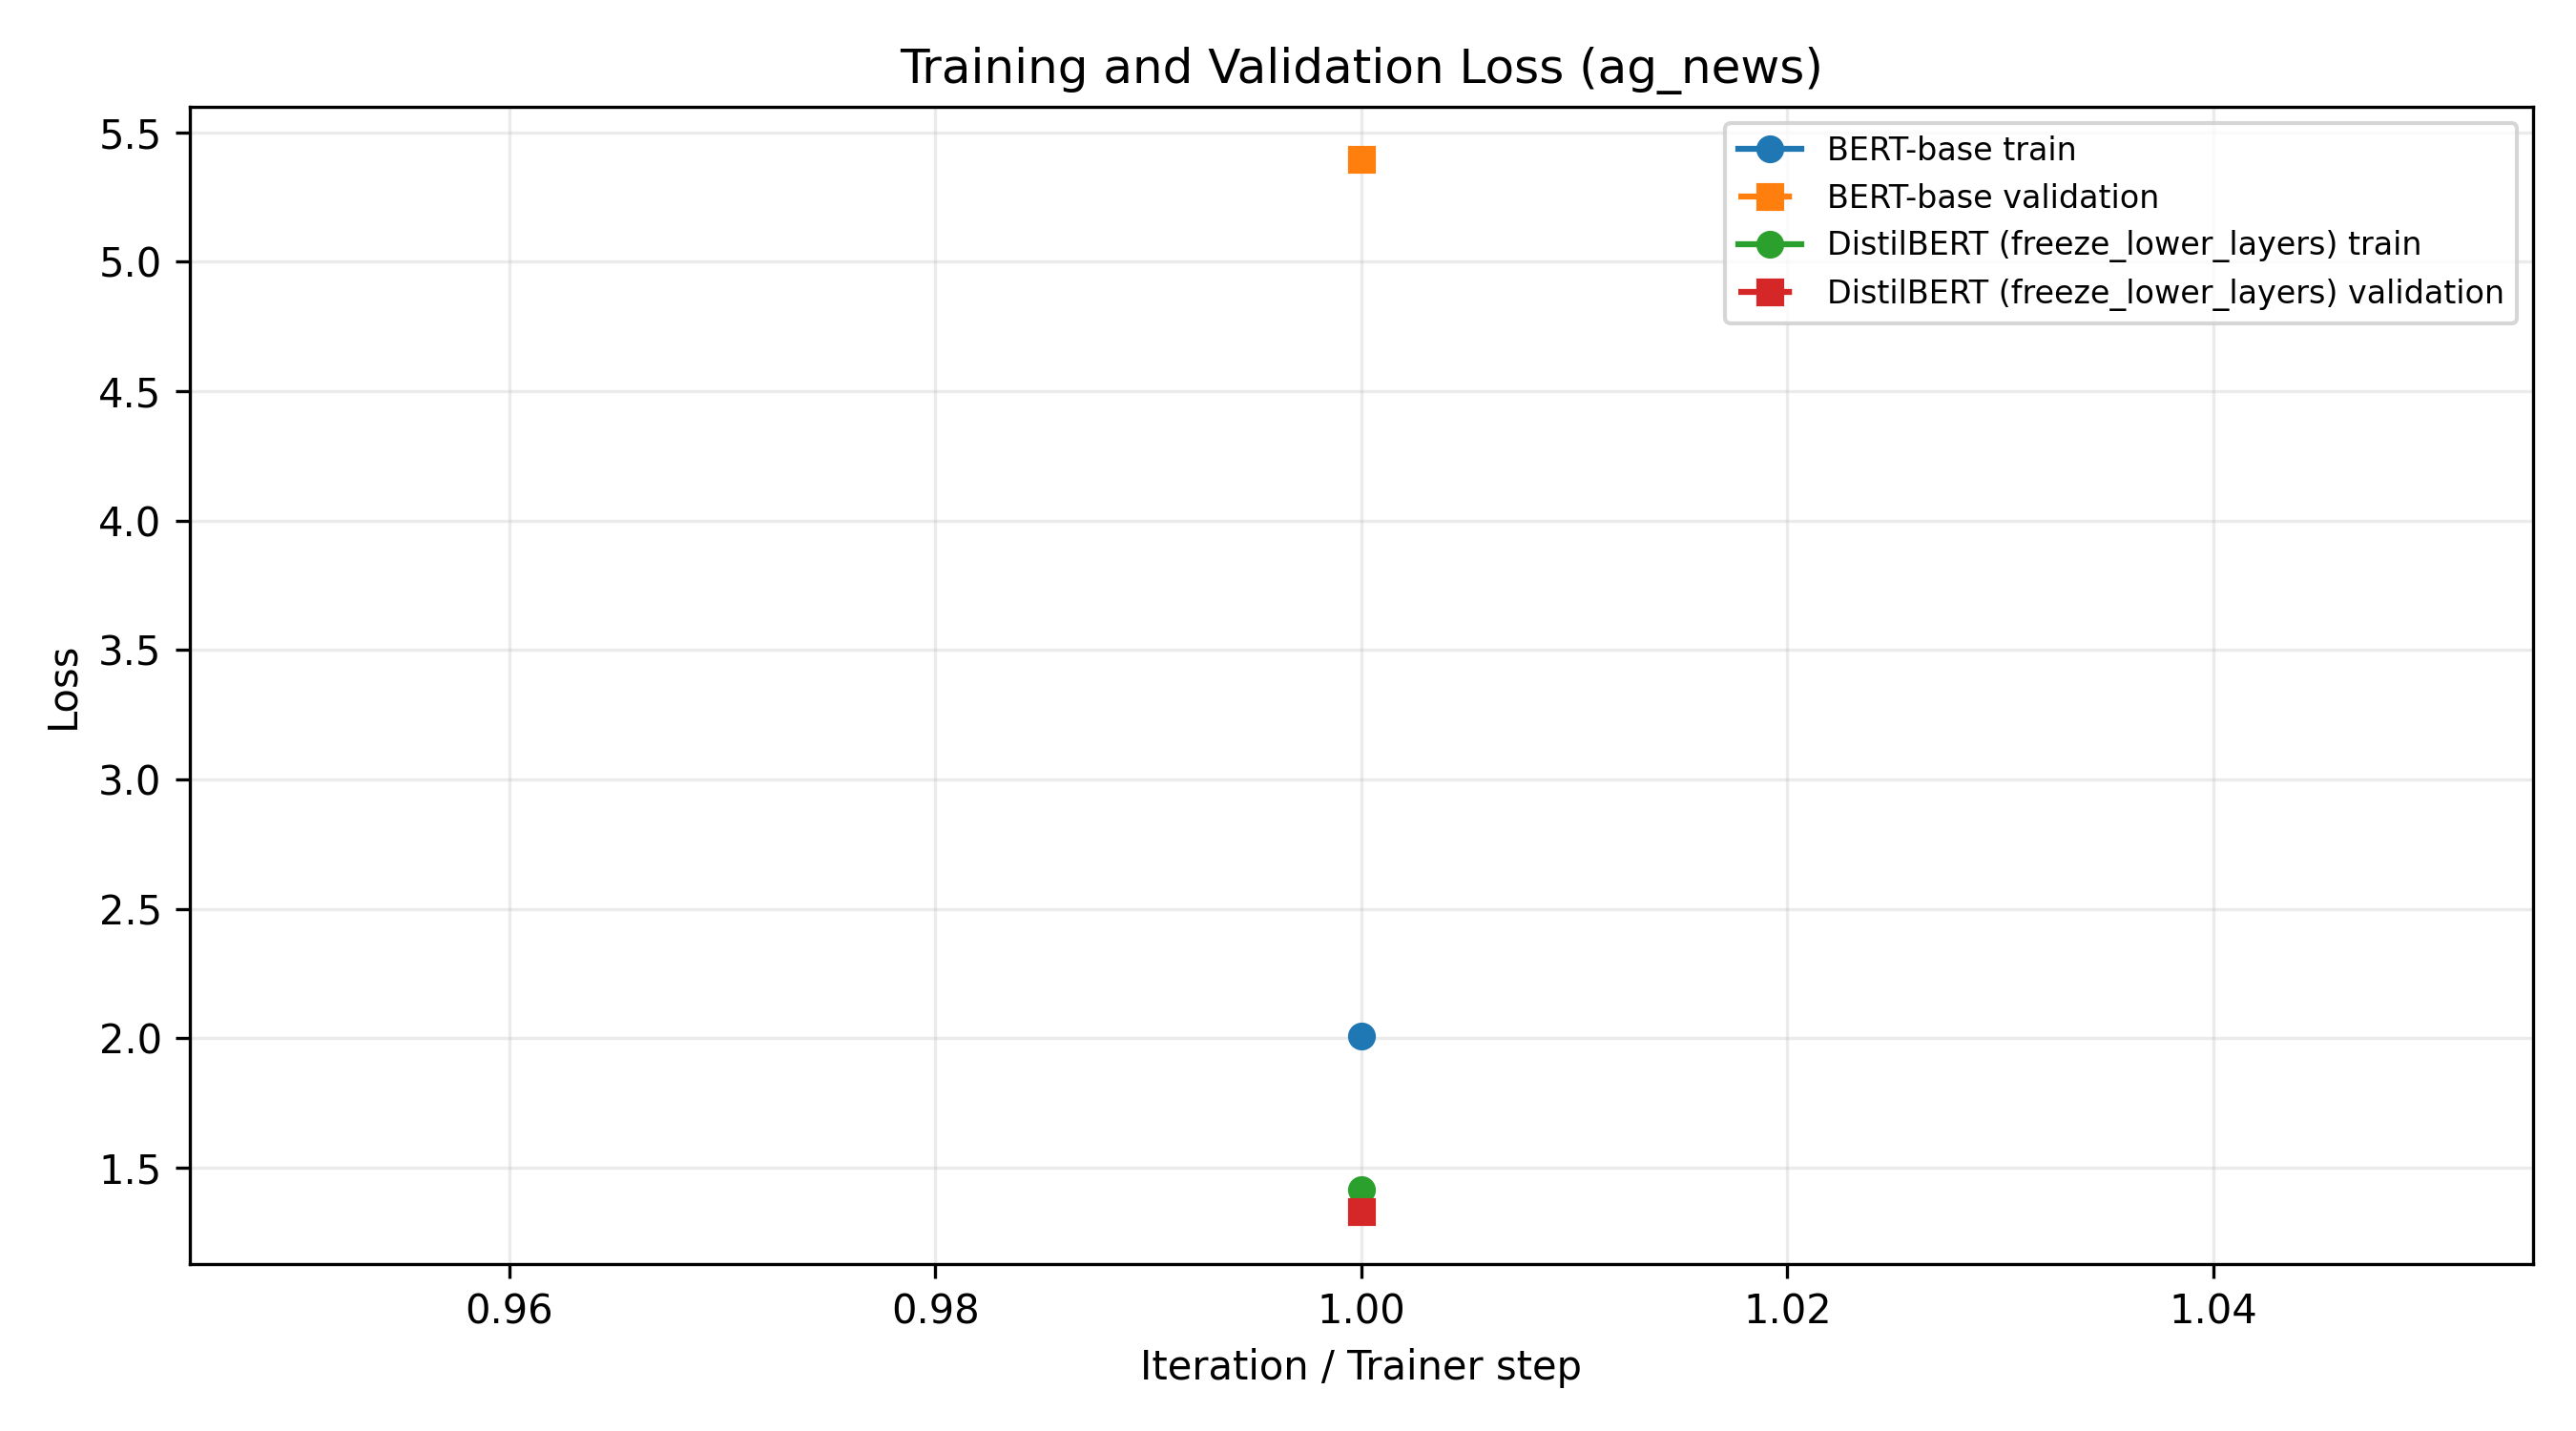
\includegraphics[width=0.32\linewidth]{figures/loss_curves_ag_news.png}
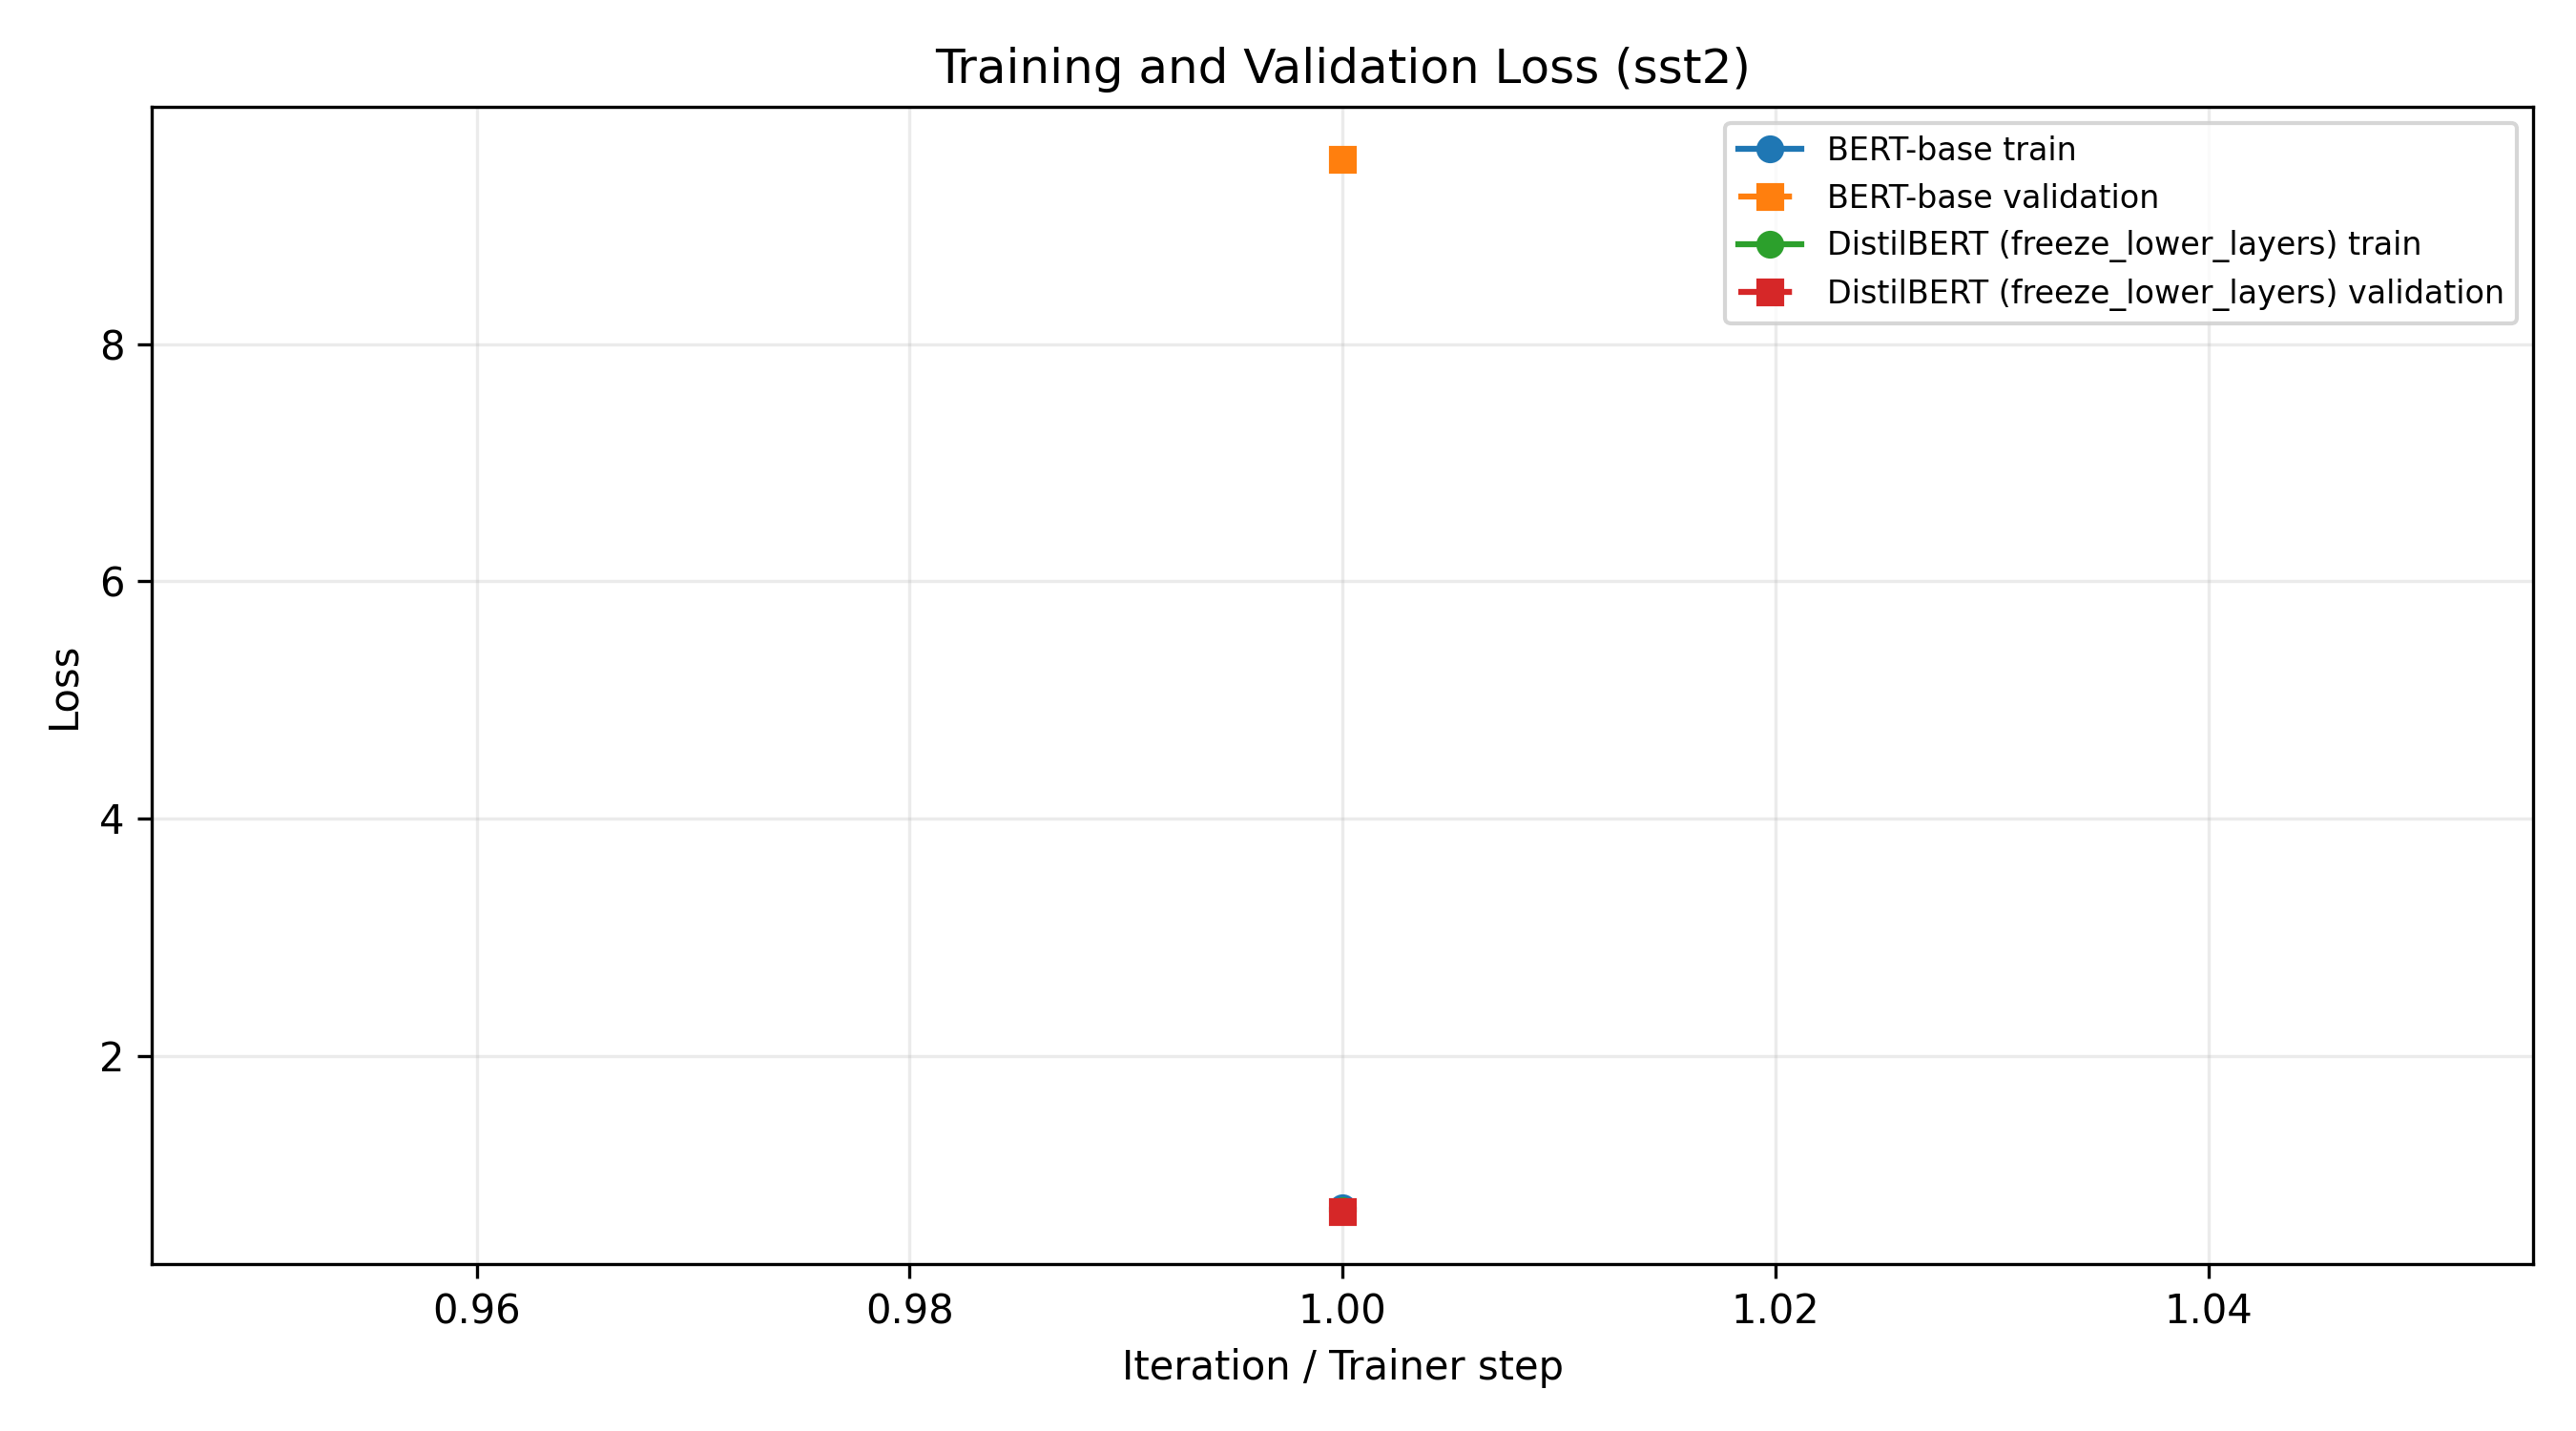
\includegraphics[width=0.32\linewidth]{figures/loss_curves_sst2.png}
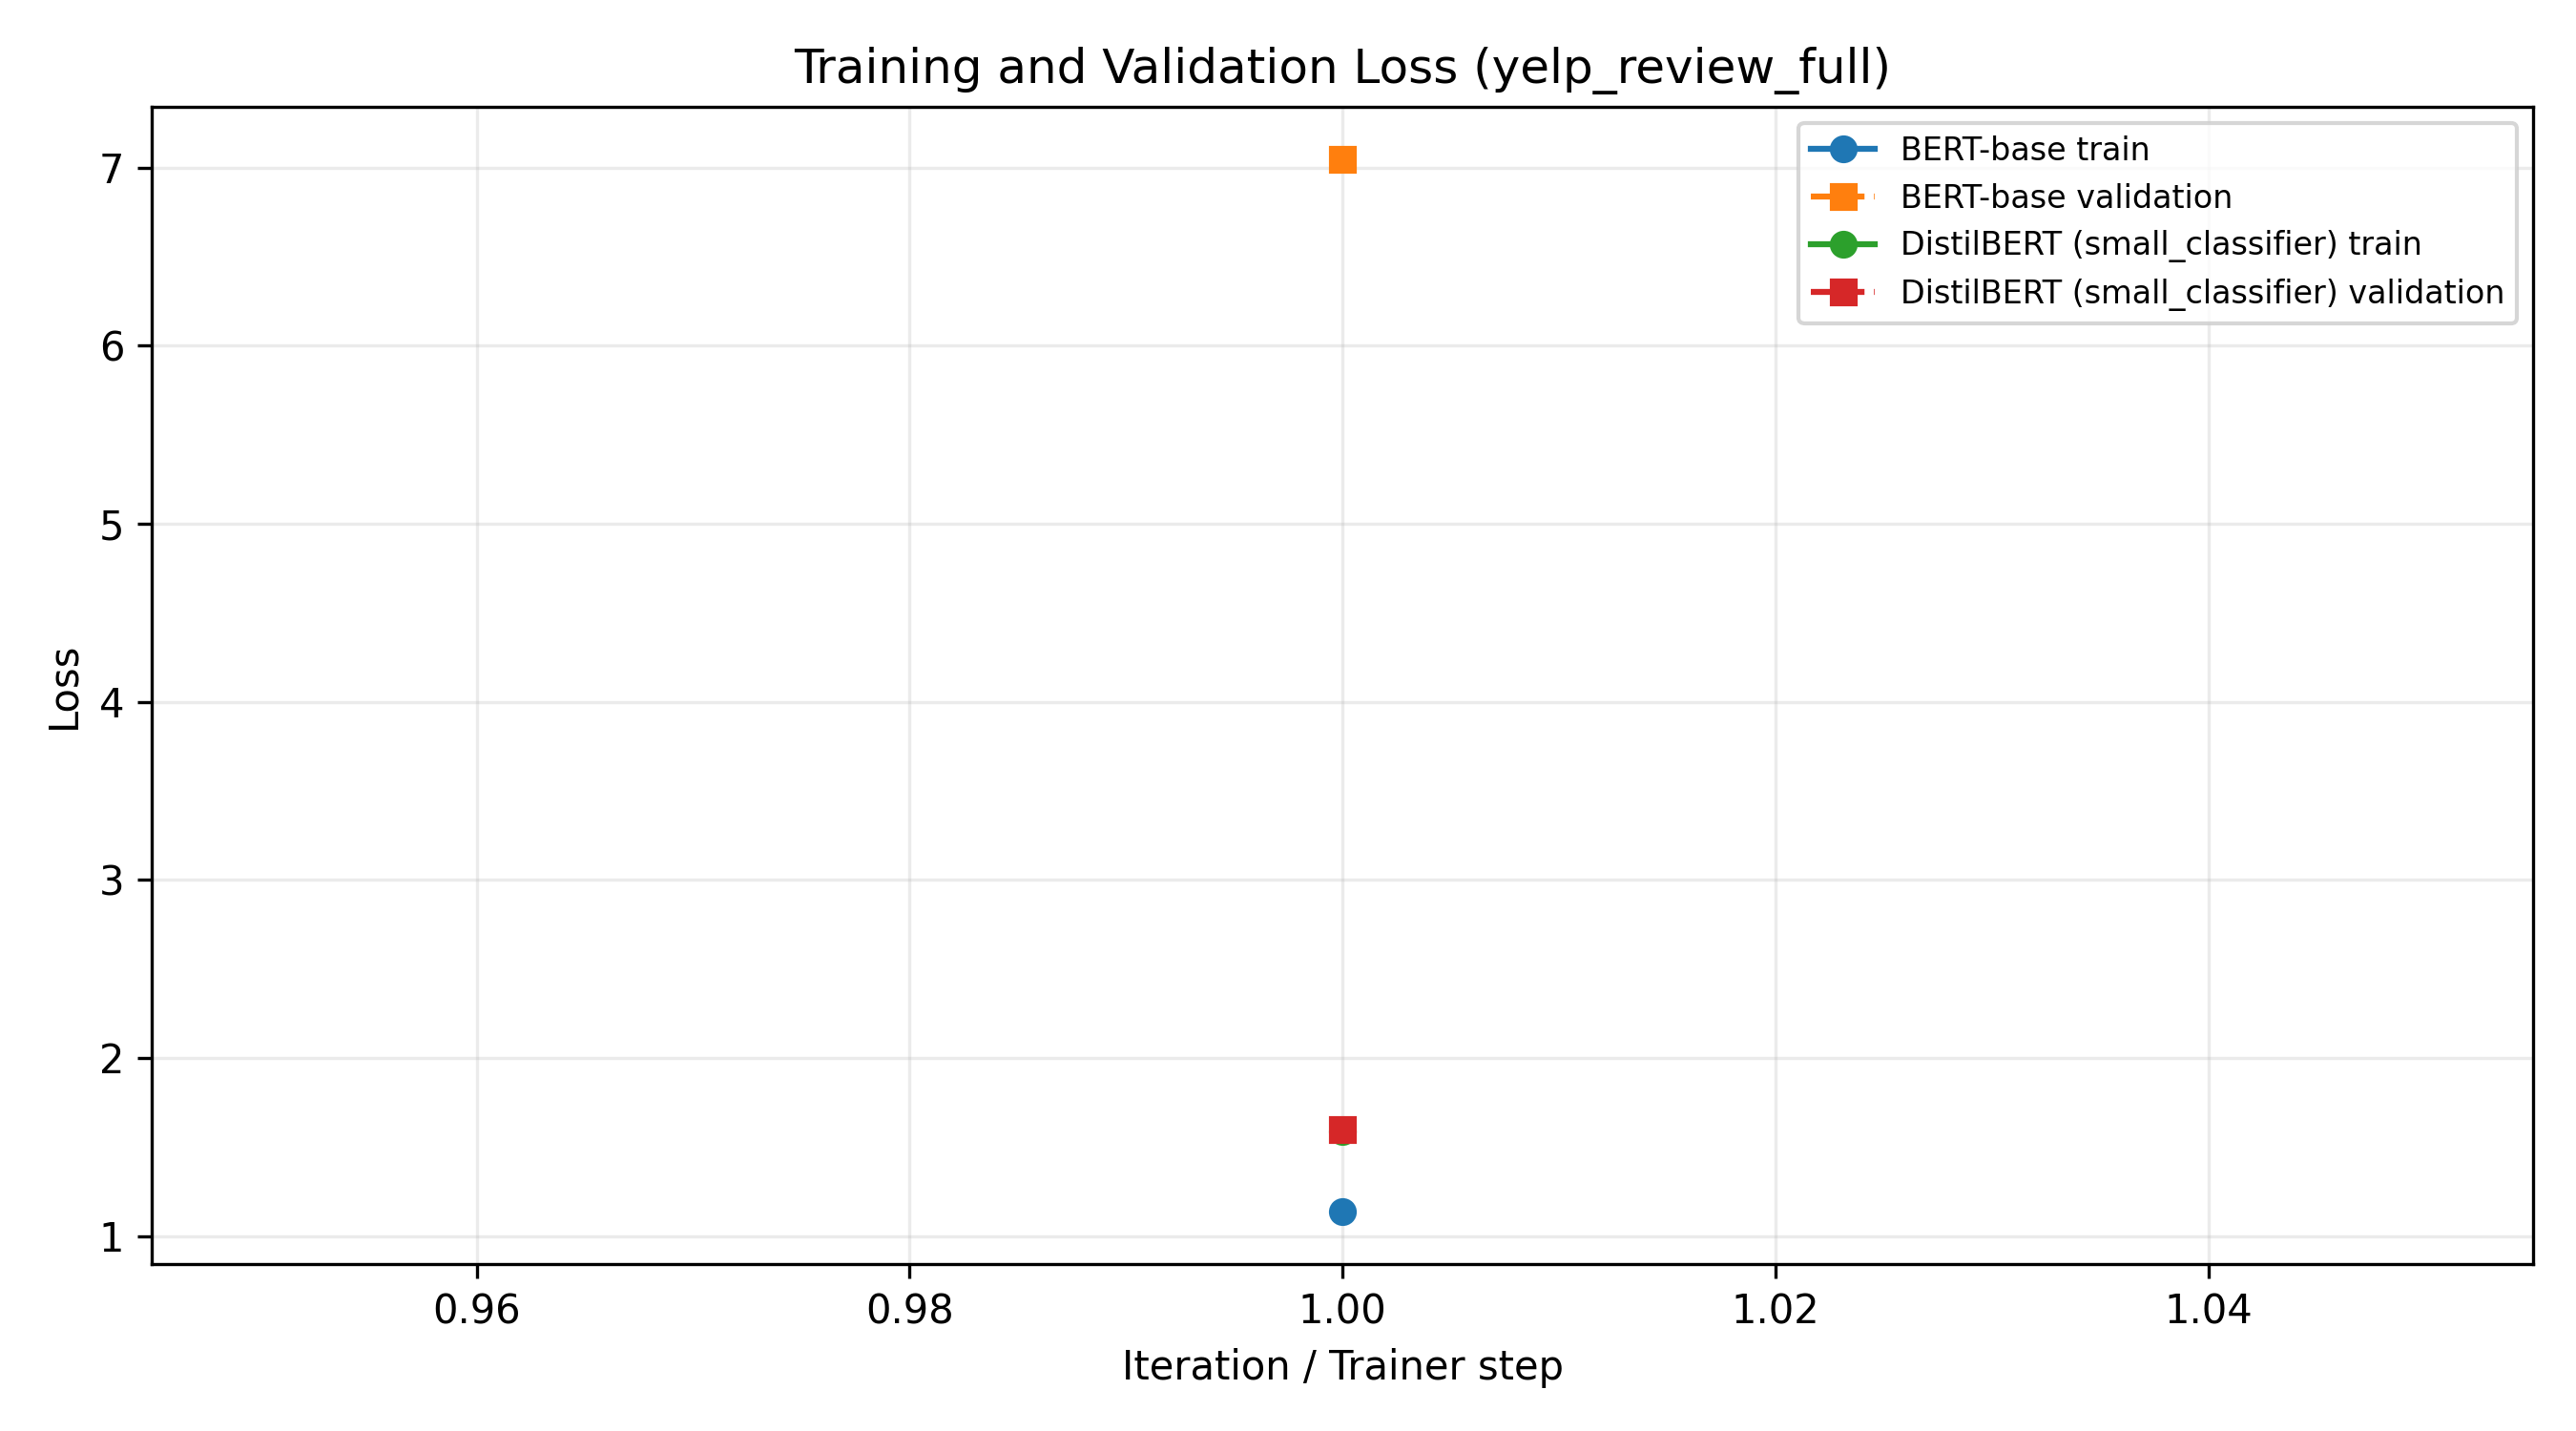
\includegraphics[width=0.32\linewidth]{figures/loss_curves_yelp_review_full.png}
\caption{Training and validation loss curves for the available final comparison runs.}
\label{fig:loss}
\end{figure}

\begin{table}[t]
\centering
\caption{DistilBERT ablation summary. To fit the mini-report format, the generated snippet keeps the top configurations per dataset.}
\label{tab:ablation}
\resizebox{\linewidth}{!}{\begin{tabular}{lllrrrrrr}
\toprule
Dataset & Config & Freeze & Head & Acc. & F1 & Params (M) & Trainable (M) & Latency \\
\midrule
ag\_news & baseline & none & [] & 0.9432 & 0.9432 & 66.96 & 66.96 & 0.18 \\
ag\_news & small\_classifier & none & [128] & 0.9412 & 0.9411 & 66.46 & 66.46 & 0.19 \\
ag\_news & large\_classifier & none & [512, 256] & 0.9393 & 0.9394 & 66.89 & 66.89 & 0.19 \\
ag\_news & freeze\_lower\_layers & lower\_layers & [256] & 0.9366 & 0.9366 & 66.56 & 21.46 & 0.18 \\
sst2 & large\_classifier & none & [512, 256] & 0.9106 & 0.9105 & 66.89 & 66.89 & 0.18 \\
sst2 & small\_classifier & none & [128] & 0.9106 & 0.9105 & 66.46 & 66.46 & 0.18 \\
sst2 & baseline & none & [] & 0.9106 & 0.9105 & 66.96 & 66.96 & 0.18 \\
sst2 & freeze\_lower\_layers & lower\_layers & [256] & 0.8784 & 0.8779 & 66.56 & 21.46 & 0.18 \\
yelp\_review\_full & baseline & none & [] & 0.6503 & 0.6502 & 66.96 & 66.96 & 0.18 \\
yelp\_review\_full & small\_classifier & none & [128] & 0.6478 & 0.6479 & 66.46 & 66.46 & 0.18 \\
yelp\_review\_full & large\_classifier & none & [512, 256] & 0.6442 & 0.6446 & 66.89 & 66.89 & 0.18 \\
yelp\_review\_full & freeze\_lower\_layers & lower\_layers & [256] & 0.6352 & 0.6347 & 66.56 & 21.46 & 0.19 \\
\bottomrule
\end{tabular}
}
\end{table}

\begin{table}[t]
\centering
\caption{Selected DistilBERT configuration per dataset.}
\label{tab:best-distilbert}
\resizebox{\linewidth}{!}{\begin{tabular}{lllrrrrrr}
\toprule
Dataset & Best config & Acc. & Prec. & Rec. & F1 & Params (M) & Trainable (M) & Latency \\
\midrule
ag\_news & large\_classifier & 0.9451 & 0.9454 & 0.9451 & 0.9451 & 66.89 & 66.89 & 0.20 \\
sst2 & large\_classifier & 0.9117 & 0.9142 & 0.9110 & 0.9114 & 66.89 & 66.89 & 0.20 \\
yelp\_review\_full & baseline & 0.6540 & 0.6548 & 0.6540 & 0.6543 & 66.96 & 66.96 & 0.20 \\
\bottomrule
\end{tabular}
}
\end{table}

The expected full-run analysis should compare whether BERT-base improves macro F1 enough to justify its larger parameter count and latency. If the selected DistilBERT configuration achieves similar F1 with fewer trainable parameters or lower latency, it is the more deployment-friendly model. If BERT-base materially improves accuracy or macro F1 on harder datasets such as Yelp Review Full, the additional compute may be justified for accuracy-critical settings. TODO: replace this paragraph with full-run findings after running the complete RTX 4090 experiments.

\section{Conclusion}
This report template completes the experimental pipeline by connecting saved metrics, plots, and tables into a NeurIPS-style mini-report. The current generated artifacts can validate the reporting workflow, but final conclusions require full-run results. The final write-up should state the best DistilBERT configuration for each dataset, whether BERT-base improves accuracy or macro F1, and whether that improvement offsets the efficiency cost. Limitations include the small model family scope, fixed maximum sequence length, and limited hyperparameter search. Future work could evaluate additional compact encoders, calibration, throughput under batching, and statistical variation across random seeds.

\bibliographystyle{plainnat}
\bibliography{references}

\end{document}
